\documentclass[a4paper]{article}
\usepackage[spanish]{babel}
\usepackage[utf8]{inputenc}
\usepackage{graphicx}
\usepackage{pdfpages}
\usepackage{enumerate}
\usepackage{listings}
\usepackage{color}
\usepackage{indentfirst}
\usepackage{fancyhdr}
\usepackage{latexsym}
\usepackage[colorlinks=true, linkcolor=black]{hyperref}
\usepackage{wrapfig}
\usepackage{algpseudocode}
\usepackage{calc}
\usepackage{amsmath, amsthm, amssymb}
\usepackage{amsfonts}
\usepackage{lscape}
\definecolor{gray}{gray}{0.5}
\definecolor{light-gray}{gray}{0.95}
\definecolor{orange}{rgb}{1,0.5,0}

\usepackage{fancyhdr}
\pagestyle{fancy}

%\renewcommand{\chaptermark}[1]{\markboth{#1}{}}
\renewcommand{\sectionmark}[1]{\markright{\thesection\ - #1}}

\fancyhf{}

\fancyhead[LO]{Sección \rightmark} % \thesection\
\fancyfoot[LO]{\small{Leandro Matayoshi, Matías Pizzagalli, Gastón Requeni, Martín Santos}}
\fancyfoot[RO]{\thepage}
\renewcommand{\headrulewidth}{0.5pt}
\renewcommand{\footrulewidth}{0.5pt}
\setlength{\hoffset}{-0.8in}
\setlength{\textwidth}{16cm}
%\setlength{\hoffset}{-1.1cm}
%\setlength{\textwidth}{16cm}
\setlength{\headsep}{0.5cm}
\setlength{\textheight}{25cm}
\setlength{\voffset}{-0.7in}
\setlength{\headwidth}{\textwidth}
\setlength{\headheight}{13.1pt}

\renewcommand{\baselinestretch}{1.1}  % line spacing


\usepackage{underscore}
\usepackage{caratula}
\usepackage{url}

\newcommand{\cod}[1]{{\tt #1}}
\newcommand{\negro}[1]{{\bf #1}}
\newcommand{\ital}[1]{{\em #1}}
\newcommand{\may}[1]{{\sc #1}}
\newcommand{\tab}{\hspace*{2em}}

\newcommand{\sprintstory}[6]{\begin{tabular}{| p{3cm} | p{12cm} |}
 \hline
 TargetProcess ID: & #1 \\
 \hline
 User Story: & #2 \\
 \hline
 Esfuerzo estimado: & #3 \\
 \hline
 Business Value: & #4 \\
 \hline
 Descripción: & #5 \\
 \hline
 Criterios de\newline Aceptación: & #6 \\
 \hline
\end{tabular}}

\newcommand{\simplestory}[5]{\begin{tabular}{| p{3cm} | p{12cm} |}
 \hline
 TargetProcess ID: & #1 \\
 \hline
 User Story: & #2 \\
 \hline
 Esfuerzo estimado: & #3 \\
 \hline
 Business Value: & #4 \\
 \hline
 Descripción: & #5 \\
 \hline
\end{tabular}}

\newenvironment{taskstable}
{ \begin{tabular}{| p{14cm} | p{1cm} |}
 \hline
 \multicolumn{2}{|c|}{{\bf División en tareas}}\\
 \hline
 {\bf Tarea} & {\bf HH}\\
 \hline }
{ \end{tabular} }

\newcommand{\task}[2]{#1 & #2\\
 \hline}

\hypersetup{
 pdfstartview= {FitH \hypercalcbp{\paperheight-\topmargin-1in-\headheight}},
 pdfauthor={Grupo},
 pdfsubject={Dise\~{n}o}
}

\lstset{escapechar=@}

\begin{document}

\thispagestyle{empty}
\materia{Ingeniería de Software II}
\submateria{Primer Cuatrimestre de 2016}
\titulo{Trabajo Práctico I: The Curry Game. Equipo: Los Pumas}

\integrante{Leandro Matayoshi}{79/11}{leandro.matayoshi@gmail.com}
\integrante{Matías Pizzagalli}{257/12}{matipizza@gmail.com}
\integrante{Gastón Requeni}{400/11}{grequeni@hotmail.com}
\integrante{Martín Santos}{413/11}{martin.n.santos@gmail.com}

\makeatletter

\maketitle

\newenvironment{myindentpar}[1]
{\begin{list}{1}
         {\setlength{\leftmargin}{#1}}
         \item[]
}
{\end{list}}

\newpage
\section{Primera parte de la entrega}
\subsubsection{Correciones respecto a la primera entrega}
Respecto a la primera entrega: 'División en user stories y backlog inicial' se corrigieron los siguientes aspectos:

\begin{itemize}
  \item Se agruparon algunas user stories (no incluídas en el sprint) en otras más generales. Los cambios están reflejados tanto en el informe como en \emph{TargetProcess}
  \item Se agregaron los títulos descriptivos en cada user story, además del \emph{targetprocess id} de cada story
  \item Se agregó el rol de \textbf{Diseñador del simulador} en reemplazo de \textbf{Diseñador del juego} en todas aquellas stories relacionadas con la simulación
  \item Se eliminaron stories relacionadas con carga manual de datos
\end{itemize}

\subsection{Introducción}
Aca va la intro =)

\subsection{Estimación de Esfuerzo}
Una vez construidas las user stories, empezamos a estimar el esfuerzo en story points. Para esto utilizamos la técnica de Planning Poker.

Primero realizamos la estimación de las historias asociadas al simulador. Cada integrante del equipo eligió un conjunto de historias 
que consideró de 1 punto de esfuerzo. Luego realizamos una puesta en común en la que estuvimos de acuerdo por unanimidad. A continuación
analizamos todas las tarjetas restantes relacionadas con la simulación y acordamos un puntaje utilizando Planning Poker. La técnica
fue muy útil para llegar a un acuerdo, ya que permitió evaluar posturas muy distintas sobre las historias. En algunos casos hubo acuerdos casi
unánimes y en otros dedicamos bastante tiempo a la discusi\'on.

Luego estimamos las historias por fuera del simulador. También comenzamos eligiendo una con esfuerzo de 1 punto y a partir de esa estimamos
el resto hasta completar el proceso.
\subsection{Estimación de Business Value}
El valor de cada story fue calculado en función de su importancia dentro del sistema. 

Dentro de las stories con más valor se distinguen 2 grandes grupos:
\begin{itemize}
  \item Aquellas relacionadas con el simulador, ya que como fue mencionado anteriormente es prioritario para el cliente
  \item Aquellas indispensables para la aplicación, sin las cuales la misma deja de tener sentido. En este caso temas de registro y login de usuarios y creación y aceptación
  de desafíos
\end{itemize}

En el nivel de \emph{great} incluímos aquellas que le dan identidad y flexibilidad a nuestro juego. En este caso, relacionadas con las apuestas de fichas en los desafíos,
y las restricciones de capital a la hora de armar los equipos.

Las stories calificadas como \emph{good} son similares a las de \emph{great} pero de menor importancia.


\newpage
\subsection{Project Backlog}
%%%%% EJEMPLOS DE USER STORY DE BACKLOG

% \simplestory
% {1}
% {Como usuario no registrado quiero ingresar mi nombre, mi cuenta de email y una contraseña para poder registrarme en la aplicación.}
% {3 pt.}
% {Nice to Have}
% {-}

%%%%%%%%%%%%%%%%%%%%%%%

\simplestory
{1}
{Como diseñador del juego quiero que se obtengan datos de popularidad en Twitter de los jugadores para afectar las fórmulas de umbral de éxito.}
{13 pt.}
{Nice to Have}
{Los datos tienen que obtenerse durante la simulación del partido y en lo posible tener en cuenta si son positivos o negativos.}

\vspace{1cm}

\simplestory
{2}
{Como participante quiero armar un equipo de basket para utilizarlo en desafíos.}
{3 pt.}
{Must Have}
% No queda muy lindo el itemize adentro de la tabla...
{\begin{itemize}
\item El equipo debe tener 5 jugadores (base, escolta, alero, ala pivot, pivot) elegidos de una lista con todos los jugadores de la liga.
\item Cada jugador de la lista permitirá acceder a su costo (valor ficticio) y a sus estadísticas.
\item Se deberá validar que no se supere el cap.
\end{itemize}}

\vspace{1cm}

\simplestory
{3}
{Como administrador del equipo quiero elegir el técnico que dirige a mi equipo para personalizar mi equipo y determinar las posibles estrategias ofensivas y defensivas.}
{2 pt.}
{Must Have}
{\begin{itemize}
\item Elegir técnico de una lista con todos los técnicos existentes en la liga.
\item Ver jugadas que tiene asociadas cada técnico.
\end{itemize}}

\vspace{1cm}

\simplestory
{4}
{Como diseñador del juego quiero cargar jugadores y sus datos estadísticos manualmente para que haya jugadores en el sistema.}
{3 pt.}
{Average}
{\begin{itemize}
\item Los porcentajes FG y 3P deben estar entre 0 y 100, APG $>=$ 0, RPG $>=$ 0, BPG $>=$ 0, SPG $>=$ 0, TO $>=$ 0, PPG $>=$ 0.
\item Se ingresan los jugadores uno por uno.
\end{itemize}}

\vspace{1cm}

\simplestory
{5}
{Como diseñador del juego quiero crear técnicos asociándolos con un libro de jugadas para que haya técnicos en el sistema}
{2 pt.}
{Average}
{-}

\vspace{1cm}

\simplestory
{6}
{Como administrador del equipo quiero ingresar un nombre para mi equipo para personalizar mi equipo.}
{1 pt.}
{Good}
{-}

\vspace{1cm}

\simplestory
{7}
{Como participante quiero guardar un equipo creado en mi lista de equipos para utilizarlo en desafíos posteriores.}
{1 pt.}
{Good}
{-}

\vspace{1cm}

\simplestory
{8}
{Como participante quiero elegir un equipo de la lista para utilizarlo en el desafìo actual.}
{1 pt.}
{Good}
{-}

\vspace{1cm}

\simplestory
{9}
{Como participante quiero ver tabla de posiciones en base a cantidad de fichas ganadas en apuestas para compararse con otros participantes.}
{2 pt.}
{Good}
{-}

\vspace{1cm}

\simplestory
{10}
{Como participante quiero ver tabla de posiciones en base a desafíos ganados/perdidos para compararse con otros participantes.}
{2 pt.}
{Good}
{-}

\newpage
\subsection{Sprint Backlog}
%%%%% EJEMPLOS DE USER STORY Y TAREAS

% \sprintstory
% {1}
% {Como usuario no registrado quiero ingresar mi nombre, mi cuenta de email y una contraseña para poder registrarme en la aplicación.}
% {3 pt.}
% {Nice to Have}
% {-}
% {\begin{itemize}
%   \item Ingresar mi nombre, mi cuenta de email y una contraseña, y apretar un botón que confirme el registro.
%   \item No debe permitir ingresar un mail sintácticamente inválido.
%   \item No debe permitir registrar dos veces el mismo mail.
%   \item La contraseña debe ser ingresada dos veces y el sistema validar que sean idénticas.
% \end{itemize}}

% \vspace{1cm}

% \begin{taskstable}
%  \task
%  {Como usuario no registrado quiero ingresar mi nombre, mi cuenta de email y una contraseña para poder registrarme en la aplicación}
%  {3}

%  \task
%  {Como usuario no registrado quiero ingresar mi nombre, mi cuenta de email y una contraseña para poder registrarme en la aplicación}
%  {3}
% \end{taskstable}

%%%%%%%%%%%%%%%%%%%%%%%%%%%%%%%%%%%%%%%%%%%%%%%%%%%%%%%%%%%%%%%%%%%%%%%%%%%%%%%%%%%%%%%%%%%%%



\newpage
\section{Segunda parte de la entrega}
\subsection{Seguimiento del Sprint}
El Sprint realizado entre el 12/04/2016 y el 04/05/2016 se completó exitosamente. Todas las user stories planificadas fueron terminadas.
A continuación presentamos los burndown charts asociados y el detalle de horas consumidas:

\begin{figure}[h!]
 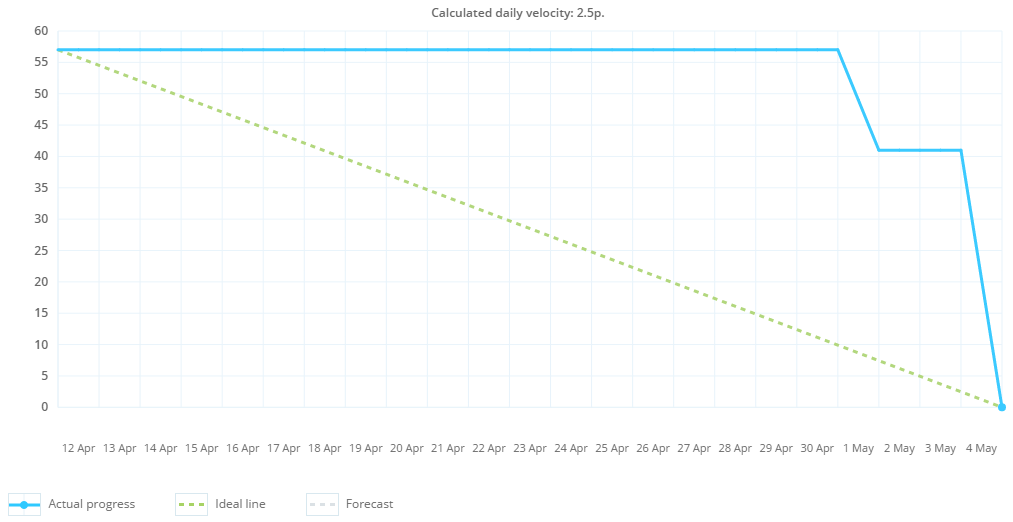
\includegraphics[width=\textwidth]{imagenes/burndown-points.png}
 \caption{Burndonw Chart de Story Points. La línea verde punteada indica el progreso ideal (comienza en 57 puntos, el total de la estimación de esfuerzo).
 La línea azul indica el progreso real.}
\end{figure}

\begin{figure}[h!]
 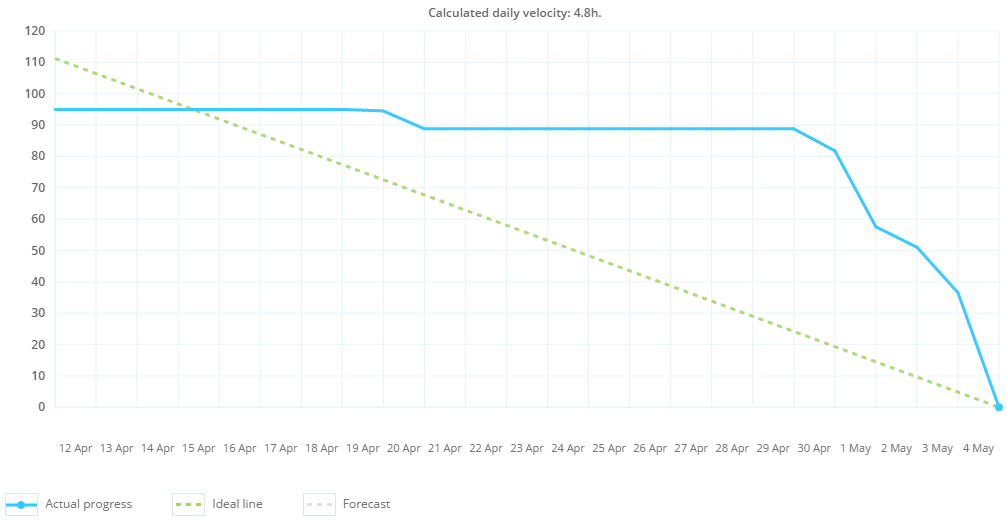
\includegraphics[width=\textwidth]{imagenes/burndown-hours.png}
 \caption{Burndonw Chart de Horas de Tareas. La línea verde punteada indica el progreso ideal (comienza en 111 horas, lo cual difiere de la estimación
 inicial de 96 horas porque se agregaron horas durante el sprint). La línea azul indica el progreso real.}
\end{figure}

En los gráficos se observa que hasta el 19/04 no hubo avance. El 20/04 se realizaron algunas tareas para discutir en la reunión con el Product Owner del
21/04. Hasta aquí no se cerró ninguna story (por eso los Story Points se mantienen constantes). En este momento se detectaron fallas en la estimación
y se agregaron horas a las tareas (es por esto que la horas empiezan estando por debajo del total de horas).

Luego hubo otro período sin avances y finalmente
a partir del 30/04 empezó a haber avance contínuo en las tareas. El 1/05 se cerró la primer user story y de ahí en más se fueron cerrando el resto.

Finalmente, la cantidad de horas hombre consumidas fue de:

\vspace{0.3cm}
\begin{tabular}{ | c | c | }
 \hline
 Horas Integrante 1: & 21\\
 \hline
 Horas Integrante 2: & 14\\
 \hline
 Horas Integrante 3: & 33.5\\
 \hline
 Horas Integrante 4: & 29.5\\
 \hline
 {\bf Horas Totales:} & 92.5\\
 \hline
\end{tabular}


\subsection{Retrospectiva}
Los atrasos fueron causados principalmente por las actividades que los integrantes realizamos además de trabajar en este proyecto. Todos
nosotros tenemos trabajos de 6hs diarias. Adem\'as uno de los integrantes dedica 10 hs por semana a la docencia y el resto est\'a cursando otra materia
en la facultad. Haciendo un balance general y teniendo en cuenta horas de descanso, por semana cada uno tuvo disponible aproximadamente 10 horas (sin
contar los fines de semana). Por último hay que tener en cuenta que la coordinación grupal se complicó por la dificultad de coincidir todos en un mismo
horario.

En conclusión, las horas netas que cada uno tuvo disponibles fueron muy pocas (en las 3 semanas del sprint, cada uno tuvo aproximadamente unas 30 hs
disponibles más fines de semana). Además hubo una semana de disponibilidad cero por el parcial, por ende sólo tiene sentido considerar
dos semanas. Esto explica claramente los saltos en los burndowns.

Para llegar a tiempo a la entrega, en el avance del 20/04 se realizó una reunión grupal para pensar un diseño a nivel global y establecer parámetros
en común. Luego se repartieron stories iniciales para cada uno (dos por persona) y se avanzó en la parte central del simulador. Cada uno fue tomando
stories extra a medida que las terminaba o que se veía imposibilitado para avanzar.

Detectamos muchas dependencias entre stories. Esto provocó que en un punto las stories estaban completamente distribuidas pero ninguna había sido
completada porque se necesitaba integración con stories de otra persona. Es por esto que muchas stories se cerraron en los últimos días, mientras
que las horas fueron disminuyendo de manera más gradual.

Al unificar las partes, detectamos ciertos problemas a solucionar en un próximo sprint:
\begin{itemize}
 \item El logger no es cerrado para la modificación cuando se quieran agregar movimientos (por ejemplo: HacerFalta).
 \item Los parámetros deben ser modificados desde la clase que los usa. Esto deberíamos abstraerlo en algúna estructura especial que pueda
 ser modificada sin afectar a los que la usan.
 \item El jugador estrella (MVP) quedó fuera de esta iteración.
 \item Las fórmulas de resolución de acciones solo tienen en cuenta las estadísticas del jugador que lleva a cabo la acción. Por ejemplo, en el caso de un tiro por tres puntos, no tomamos en cuenta la cantidad de pases que se hicieron previamente. Esto es algo a resolver en la siguiente iteracion.
\end{itemize}

\section{Interacciones dentro del simulador}
\subsection{Aclaraciones}
En algunas de las secciones siguientes utilizamos pseudocódigo para acompañar las explicaciones. Para ello utilizamos el package 'algpseudocode'. 
El mismo define funciones con una estructura \textbf{function} \ldots \textbf{end function}. Si bien esa sintaxis no expresa correctamente la idea de mensajes
utilizada por el paradigma orientado a objetos ya que no estamos definiendo 'funciones' si no respuestas a envíos de mensaje, utilizamos dicho paquete por cuestiones
de estilo y prolijidad. La palabra \textbf{funcion} debe ser entendida como \textbf{mensaje}.

\subsection{Defendiendo un movimiento ofensivo}
\subsection{Defendiendo un movimiento ofensivo}

Se puede pensar que en el basket existe una acción contraria a cada movimiento ofensivo. Para el pase existe la intercepción y para el tiro el bloqueo. (El rebote no es considerado
movimiento ofensivo). Por lo tanto, las jugadas defensivas tienen la oportunidad de responder con una secuencia de acciones defensivas (puede ser una o muchas) ante cada movimiento
ofensivo. En el caso de una jugada defensiva hombre a hombre, cada acción de un jugador ofensivo en una posición determinada es defendida por una única acción 
contraria realizada por el jugador en la misma posición del equipo rival. Sin embargo, podría existir una jugada defensiva que marque únicamente los tiros de 3 puntos pero cada uno de ellos
con varios jugadores. Es por eso que cada acción ofensiva puede ser defendida con una serie de movimientos.

La jugada defensiva recibe el mensaje defender, pero en un principio desconoce \emph{qué} acción debe defender. Para evitar el uso de \textbf{if} se utiliza el double dispatch.
Al objeto pasado por parámetro se le envía el mensaje \emph{informarTipoDeMovimiento}.

\newpage
\begin{landscape}

  \begin{figure}[h!]
   \includegraphics[scale=0.35]{imagenes/defender-pase.png}
   \caption{}
  \end{figure}

\end{landscape}
\newpage


\subsection{Eligiendo jugada ofensiva}
Al momento de elegir una jugada ofensiva el técnico la selecciona de su libro de jugadas. El mismo tiene como colaboradores internos dos arreglos de 
GeneradoresDeJugada: uno para las ofensivas y otro para las defensivas. 

Introducimos una clase 'Generador*' por el siguiente motivo:
Las jugadas ofensivas tienen como colaborador interno a un jugador que indica quien es el portador actual del balón y opcionalmente otros colaboradores como la
cantidad de pases realizada hasta el momento. En el caso de que se produzca un reboteo en donde el mismo equipo 
atacante vuelva a ganar la posesión del balón la jugada debería resetearse. Es decir, volver a un estado inicial. 
En lugar de hacer eso, preferimos que cada vez que el técnico seleccione una jugada se genere una nueva instancia de la misma.
Para eso usamos precisamente un 'GeneradorDeJugadaX' donde X es una jugada tanto ofensiva como defensiva.

El generador tiene además como colaborador un objeto de clase 'frecuenciaDeUso', que es utilizado por un objeto generadorDeNumerosAleatorios que determinará 
de forma random la jugada seleccionada.

Si bien una jugada \emph{defensiva} no tiene el problema de mantener un estado (con lo cual no tiene el problema de tener que resetearse),
diseñamos la elección de las mismas a través de objetos generadores también porque comparten el hecho de tener una 'frecuenciaDeUso', y para lograr que la elección
de ambos tipos de jugadas sea análogo.

\begin{figure}[h!]
   \includegraphics[scale=0.45]{imagenes/elegir-jugada-clases.png}
   \caption{Diagrama de clases en donde se muestra el tecnico, su libro de jugadas, los generadores de las distintas jugadas y las clases de las jugadas}
\end{figure}

En resumen, los generadores son los encargados de generar las nuevas instancias de las jugadas elegidas por los técnicos. A continuación se muestra un diagrama
de secuencia en donde se muestran las interacciones que entran en juego desde el momento en que se le informa al técnico que debe elegir una jugada ofensiva.
El número aleatorio obtenido es menor a la frecuencia de uso del generadorDeJugadaOfensivaDe3PuntosKPases. El técnico utiliza dicha jugada el 70\% de las veces,
por lo que dicho generador es seleccionado
como jugada seleccionada por el técnico del equipo 'Los Pumas'. Finalmente se le envía el mensaje 'crearJugada' al generador para que devuelva una instancia
de JugadaOfensivaDe3PuntosKPases.
Si bien en la secuencia se selecciona una jugada ofensiva, la elección de jugada defensiva es análoga por lo que no se muestran diagramas para ello.

~

En el diagrama de secuencia hay una colaboración entre el técnico de Los Pumas y el equipo Los Pumas en donde no aparece el nombre del mensaje que se envía.
Esto se debe a que el equipo es un colaborador interno del técnico. Sin embargo, la flecha fue agregada para indicar que se produce una colaboración entre
ambos objetos.

\newpage
\begin{landscape}

\begin{figure}[h!]
   \includegraphics[scale=0.27]{imagenes/elegir-ofensiva.png}
   \caption{Contexto: El técnico de Los Pumas elige una jugada ofensiva. El generador obtenido es el de JugadaOfensivaDe3PuntosKPases, el cual se utiliza para
   generar una JugadaOfensivaDe3PuntosKPases}
\end{figure}

\end{landscape}
\newpage


\subsection{Movimientos ofensivos y defensivos}
El funcionamiento de un pase se encuentra fuertemente relacionado con una acción defensiva.
Un pase no va a tener éxito si una intercepción se lo impide. Este comportamiento se puede extender a cualquier movimiento ofensivo del juego.
Es por este motivo que tomamos la decisión de encapuslar este comportamiento de acción-reacción dentro de cada movimiento ofensivo
de manera que una acción ofensiva tenga éxito solo si la acción ofensiva tiene éxito y además la defensiva falla. 

Para los movimientos defensivos tenemos un comportamiento distinto. Ya no existen acciones que las contrarresten, no hay reaccion frente a ellas.
Si son exitosas, se ejecutan desde el contexto de un movimiento ofensivo. 

Para modelar el comportamiento descripto realizamos el siguiente diseño:

\begin{figure}[h!]
  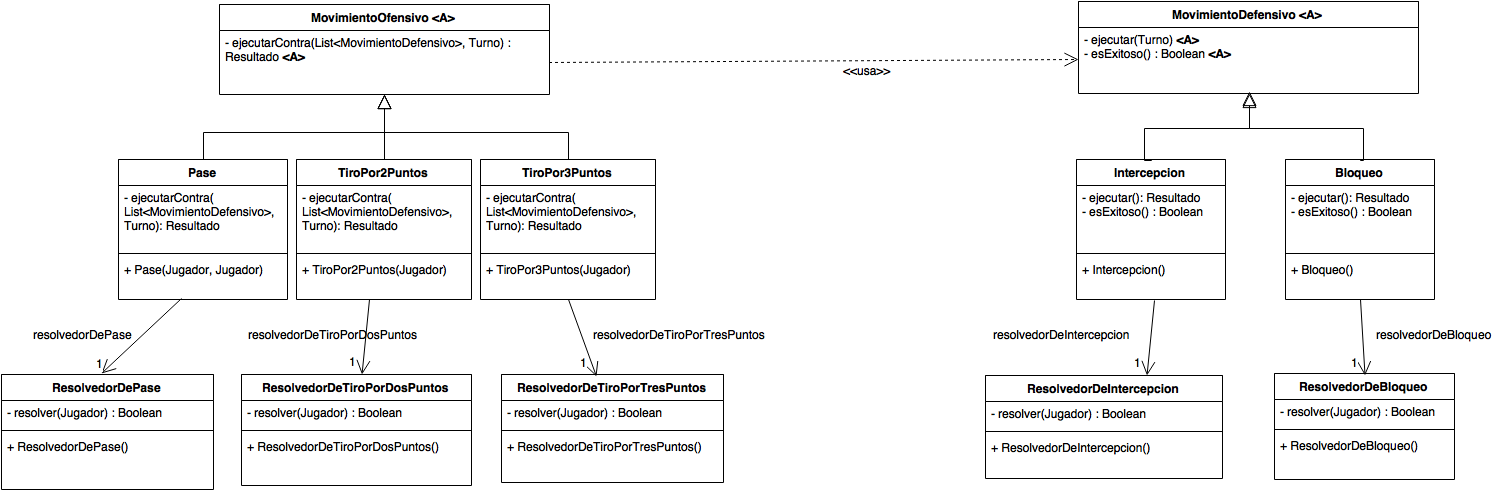
\includegraphics[scale=0.30]{imagenes/diagrama-clases-movimiento.png}
  \caption{Diagrama de clases para los movimientos ofensivos y defensivos}
\end{figure}

Para modelar el comportamiento común entre los movimientos ofensivos creamos una clase abstracta MovimientoOfensivo que sabe responder al mensaje ``ejecutarContra(unaAccionDefensiva)''. En el caso de los movimientos defensivos creamos una clase absracta MovimientoDefensivo que sabe responder a ``ejecutar()'' y ``esExitoso()''. 

A continuación, un diagrama de secuencia que representa la ejecución de un movimiento ofensivo, en este caso un pase exitoso.
Si bien no llega a mostrarse en el diagrama, el turno es el encargado de orquestar esta interacción entre movimiento ofensivo y defensivo, por lo que le envía a los 
diferentes movimientos ofensivos el mensaje 'ejecutarContra'. Este es el pseudocódigo de la implementación del mensaje \textbf{proxima\_accion} en la clase 'Turno'

~

\begin{algorithmic} 
  \State $accionOfensiva\gets jugadaOfensiva.proximoMovimiento$
  \State $accionesDefensiva\gets jugadaDefensiva.defender(accionOfensiva)$
  \State $\wedge \ accionOfensiva.ejecutarContra(accionesDefensivas)$
\end{algorithmic}

 
\begin{landscape}

  \begin{figure}[h!]
   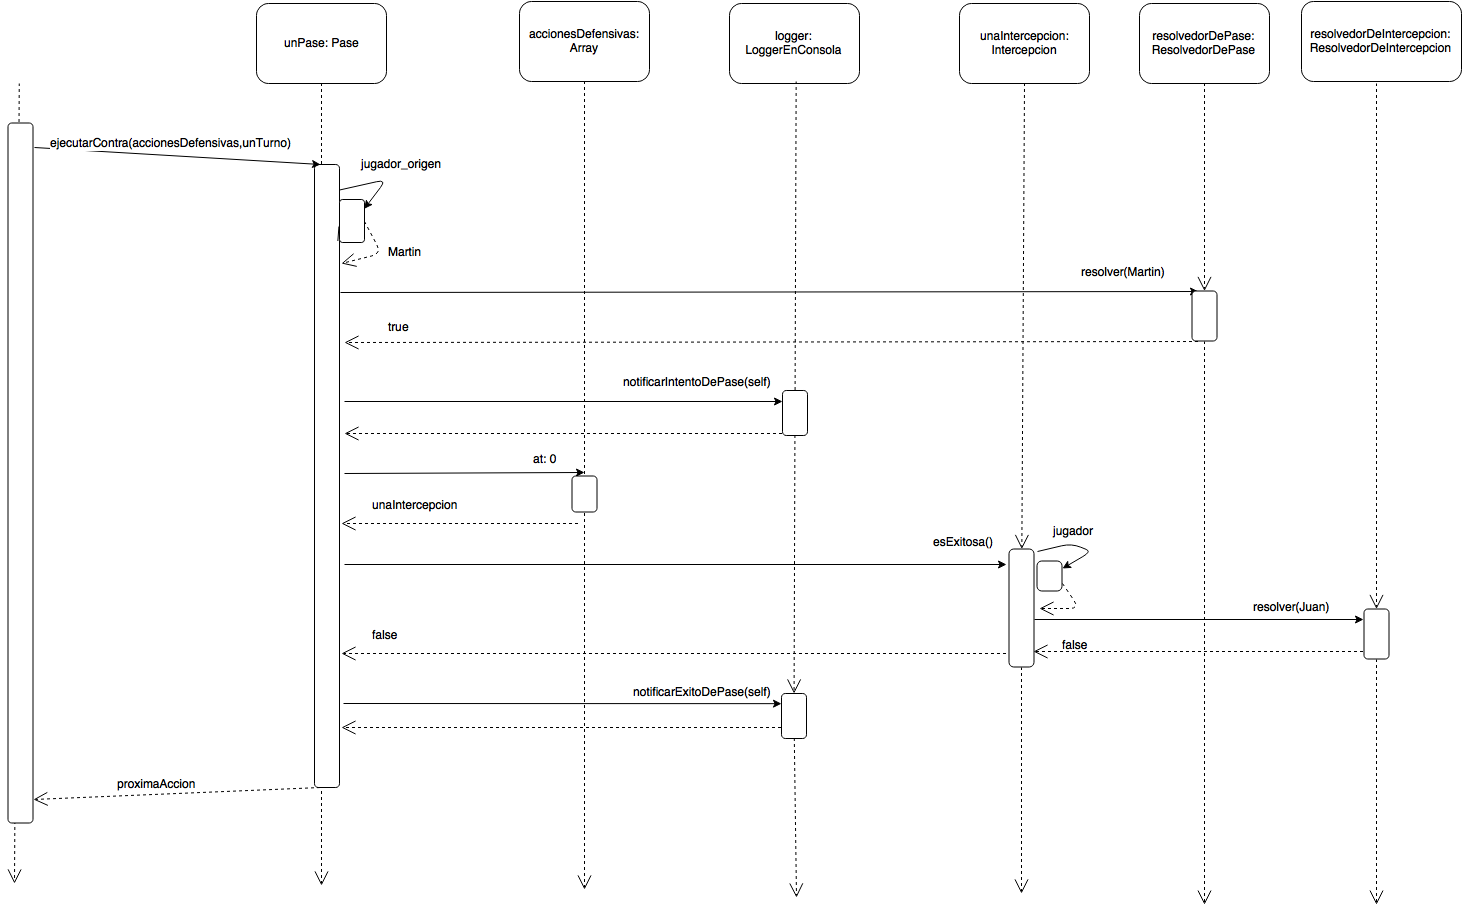
\includegraphics[scale=0.35]{imagenes/pase-exitoso.png}
   \caption{Un pase exitoso. Aclaración: se asume que el array de jugadas defensivas está compuesto por un único elemento para simplificar el diagrama.}
  \end{figure}

\end{landscape}


\subsection{Pase ficticio instantáneo al comenzar nueva jugada}
En la simulación no abstrajimos en una clase el concepto de pelota, sino que son las jugadas ofensivas quienes determinan quien tiene la pelota en un momento determinado.

Las jugadas ofensivas inicializan un colaborador interno portadorDelBalon al ser instanciadas, que representa el jugador que debe arrancar con la pelota.
A medida que se realizan pases dicho portador se va actualizando y el receptor del pase se convierte en el nuevo portador.
Sin embargo, durante la ejecución de un turno pueden suceder eventos relacionados con la recuperacion del balon(intercepción exitosa u obtención de rebote)
que obliguen a los técnicos a elegir nuevamente una jugada para el mismo turno que sigue corriendo. Al analizar la jugada ofensiva
elegida no es posible asegurar que el portadorDelBalon inicial se corresponda con el portador del balon en el contexto de la ejecución del turno. 

Resulta más fácil explicar este hecho mirando el siguiente pseudocódigo, analizando por ejemplo los eventos al ocurrir un cambio de posesión:

~

\underline{En la clase \textbf{Turno}}

~

\begin{algorithmic}
	\Function{cambio\_de\_posesion}{equipo\_ofensivo, equipo\_defensivo}
	  \State $self.equipo\_ofensivo\gets equipo\_ofensivo$
	  \State $self.equipo\_defensivo\gets equipo\_defensivo$
	  \State $elegir\_jugadas$
	  \State $proxima\_accion$
	\EndFunction
\end{algorithmic}

~ 

Una acción que puede notificarle a un turno acerca de un cambio de posesion es por ejemplo una intercepción realizada por un jugador. Supongamos la intercepción del Alero de un equipo.

~

\underline{En la clase \textbf{Intercepcion}}

~

\begin{algorithmic}
	\Function{ejecutar}{unTurno}
	  \State \ldots
	  \State unTurno.cambio\_de\_posesion(self.jugador.equipo, self.jugador.equipo.oponente)
	  \State \ldots
	\EndFunction
\end{algorithmic}

~

En ese contexto, la acción inicial de la jugada elegida puede ser un pase entre el Base y el Escolta del equipo que ha interceptado recientemente la pelota (muchas jugadas
del basket empiezan con el base como portador inicial), cuando en realidad la intercepción pudo haber sido lograda por el Alero del equipo. Es como si la pelota se teletransportara
directamente al portadorDelBalon inicial de la jugada seleccionada.

Elegimos esta opción para facilitar la implementación y considerando el hecho de que lo mismo sucede para ambos equipos, por lo que no debería tener grandes repercusiones en la 
simulación de un desafío.


\subsection{Log de Simulación}
El log de simulación debe permitir registrar todos los eventos interesantes de la simulación como inicio y fin del partido o de un turno,
intento de movimiento y su resultado (exitoso o fallido), etc. Los eventos a loggear en principio serán siempre los mismos, pero eventualmente
podría cambiar la representación del log (un archivo, impresión por consola, un objeto especial, etc). Estas ideas están reflejadas en la
intención del patrón de diseño \emph{Builder}. En nuestro caso, el builder es el {\tt Logger} y el producto será una impresión por consola, un 
{\tt Archivo}, etc. El director está distribuído entre los movimientos defensivos y ofensivos, reboteo y turno.

A continuación presentamos el modelado de clases del log de simulación:

\begin{figure}[h!]
  \includegraphics[scale=0.35]{imagenes/clases-logger.png}
  \caption{Logger usando el patrón \emph{Builder}}
\end{figure}

El Turno es el director principal (al enviar el mensaje ``comenzar()'' este se encarga de ejecutar jugadas y movimientos). Adem\'as provee
el mensaje ``logger()'' para que los movimientos y jugadas puedan enviar mensajes al logger.

El logger se instancia desde el subsistema de desafíos. Cuando a un objeto desafío se le envía el mensaje ``simular()'', se realiza lo siguiente:


\begin{algorithmic} 
	\State ...
	\State Logger $logger$ = new LoggerEnArchivo()
	\State Simulador simulador = new SimuladorDeBasket()
	\State ResultadoDto res = simulador.simular(equipoDto1, equipoDto2, $logger$)
	\State Archivo logDeSimulacion = $logger$.archivo()
	\State ...
\end{algorithmic}

De esta manera obtiene el log final, que dependerá del logger que se haya utilizado.


\subsection{Reboteo}
La acción de reboteo es un movimiento particular en el contexto de un partido de basquet. No se trata de un movimiento ofensivo ni defensivo.
Representa el caso en donde todos los jugadores intentan hacerse con el balón que se encuentra en el aire. Como se trata de un comportamiento nuevo decidimos
modelarlo de la siguiente manera:

\begin{figure}[h!]
  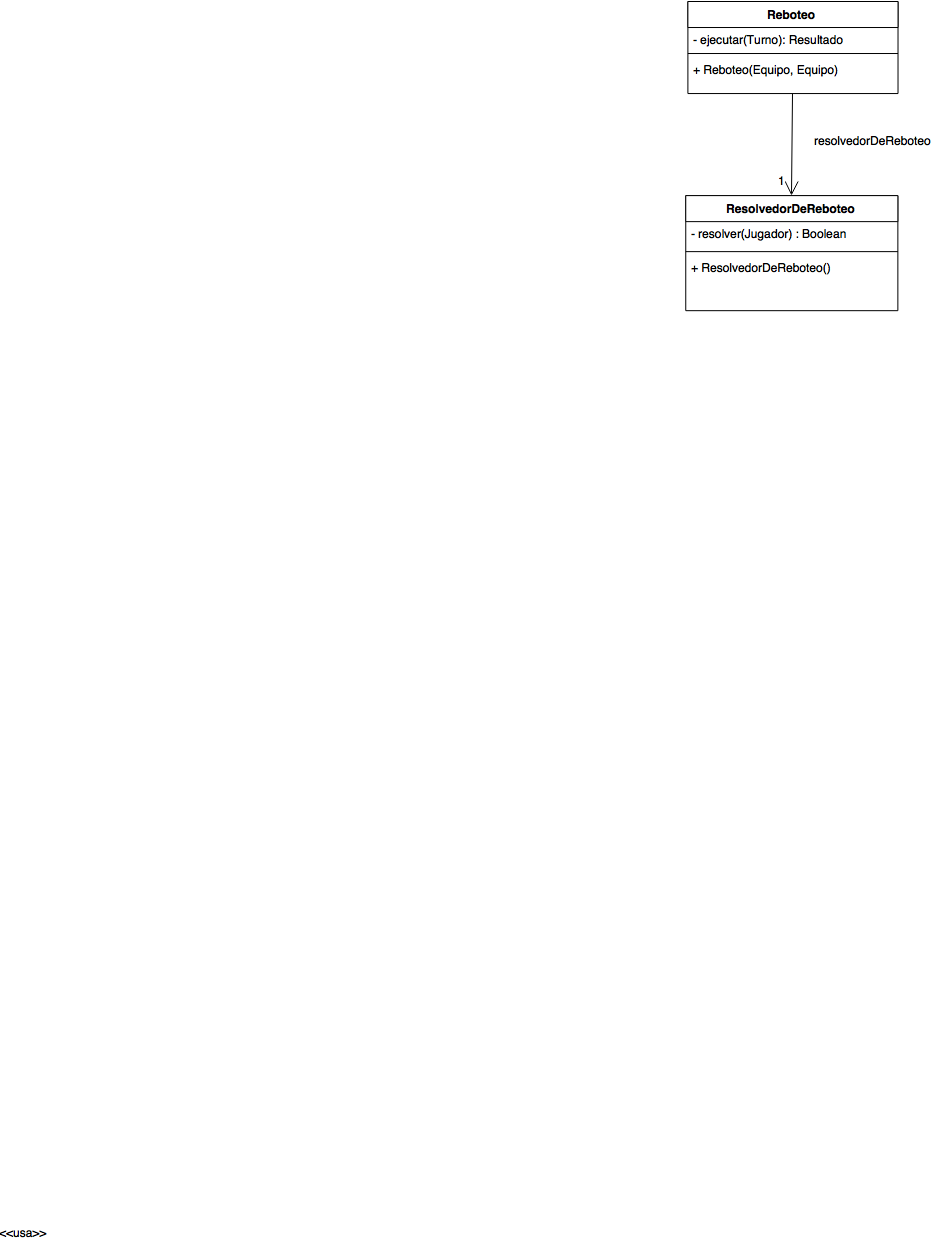
\includegraphics[scale=0.25]{imagenes/diagrama-clases-reboteo.png}
  \caption{Diagrama de clases para el movimiento de reboteo}
\end{figure}

A continuación, un diagrama de secuencia que representa la ejecución de un reboteo.

\begin{landscape}

  \begin{figure}[h!]
   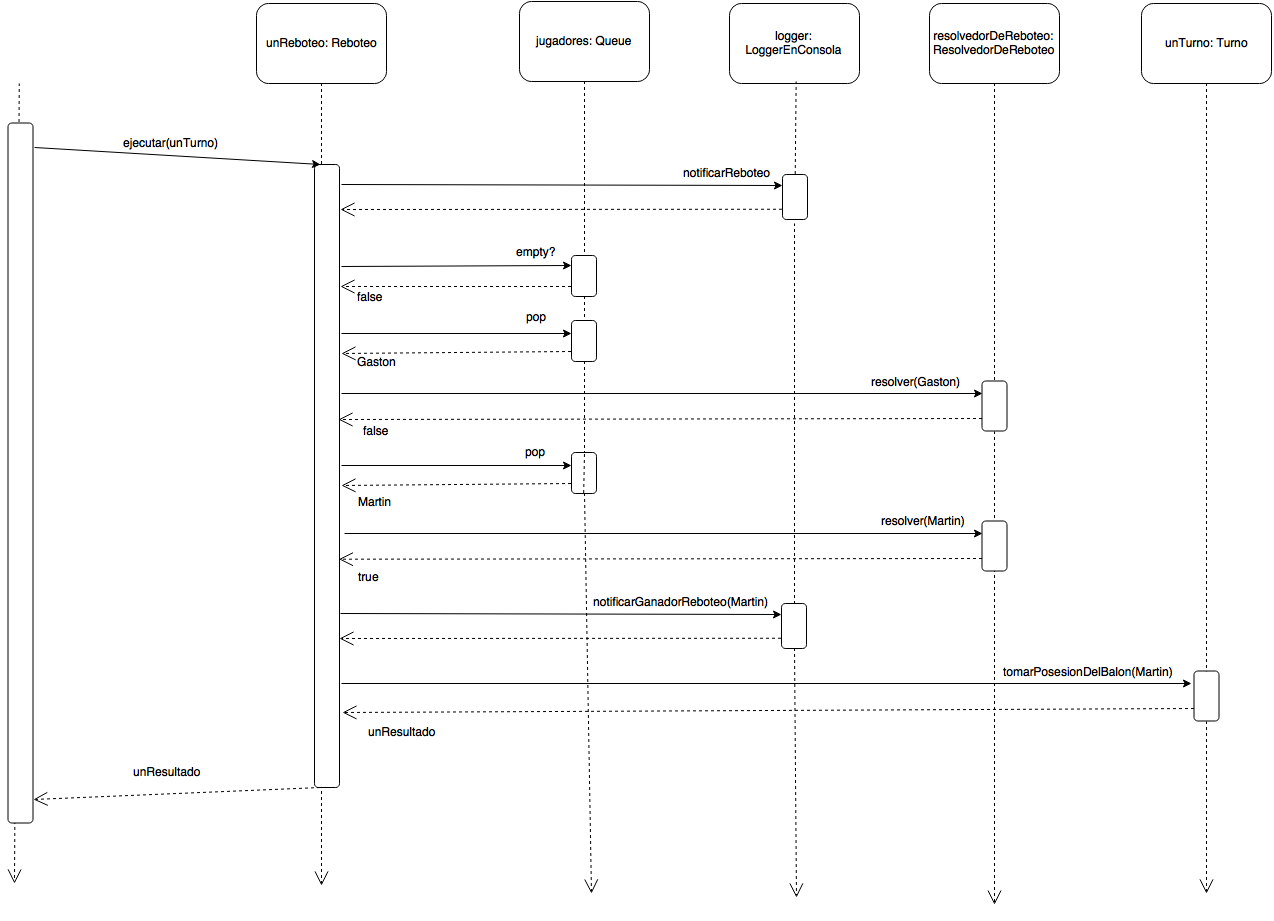
\includegraphics[scale=0.35]{imagenes/reboteo.png}
   \caption{Un reboteo cuyo ganador es Martin.}
  \end{figure}

\end{landscape}




\subsection{Subsistema de Desafíos}
El subsistema de desaf\'ios modela los participantes, el armado de equipos con jugadores reales, apuestas con fichas y creaci\'on y ejecuci\'on
de desaf\'ios.

Los jugadores reales representan a los posibles jugadores que se pueden usar para armar equipos. Los Equipos reales son los equipos de la liga.

A continuaci\'on presentamos el diagrama de clases y explicaremos la resoluci\'on de los principales casos de uso.

\newpage
\begin{landscape}

  \begin{figure}[h!]
   \includegraphics[scale=0.35]{imagenes/clases-subsistema-desafios.png}
   \caption{}
  \end{figure}

\end{landscape}
\newpage


\subsubsection{Participante}
Un participante se crea con un {\tt Nombre}, {\tt Mail} y {\tt Password} que son esenciales al participante y serán inmutables en este modelo.
El método de creación de instancia es el siguiente:

\begin{algorithmic}
	\Function{Participante}{Nombre unNombre, Mail unMail, Password unaPassword}
	  \State nombre = unNombre
	  \State mail = unMail
	  \State password = unaPassword
	  \State cap = new Capital(CAP\_INICIAL)
	  \State fichasDisponibles = new CantidadDeFichas(FICHAS\_INICIALES)
	  \State equiposGuardados = [\ ]
	  \State desafiosAbiertos = [\ ]
	  \State desafiosGanados = [\ ]
	  \State desafiosPerdidos = [\ ]
	\EndFunction
\end{algorithmic}

CAP\_INICIAL y FICHAS\_INICIALES son constantes predefinidas en la clase.

\begin{figure}[h!]
   \includegraphics[width=\textwidth]{imagenes/clases-participante.png}
   \caption{Modelado de Participantes}
\end{figure}

\subsubsection{Armar equipos}
Para armar equipos existe la clase {\tt ConstructorDeEquipos} que contiene la lógica de control de capital. Se inicializa con un Participante (que
conoce su capital) y luego se
van eligiendo jugadores. Cada vez que se elige un jugador, se resta el costo del jugador al capital ($unJugadorReal.costo$) y se actualiza el saldo
restante en un contador interno. Si el jugador
es reemplazado por otro, primero se suma el costo del jugador que se saca y se resta el que se pone (usando los mensajes ``restar(Costo)'' y ``sumar(Costo)''
de la clase {\tt Capital}).

Si se intenta restar un costo mayor al capital disponible, el método de ``restar(Costo)'' lanza una excepción que será elevada al método que llamó
al {\tt ConstructorDeEquipos}, informando la imposibilidad de comprar ese jugador por falta de fondos.

El mensaje ``comprar()'' retorna el equipo armado.

Los jugadores reales, sus costos y estadísticas se pueden acceder a partir de los equipos reales {\tt EquipoReal} que representan los equipos de la 
liga real.

Una vez que el equipo fue armado, se puede usar para crear un desafío o para guardarlo para uso futuro. En el primer caso, se utiliza el mensaje
``unParticipante.crearDesafio(unEquipoParticipante, unaApuesta)'', mientras que en el último, se usa el
mensaje ``unParticipante.guardarEquipo(unEquipoParticipante)''.

\begin{figure}[h!]
   \includegraphics[width=\textwidth]{imagenes/clases-armar-equipos.png}
   \caption{Modelado del ConstructorDeEquipos}
\end{figure}

\begin{algorithmic}
	\Function{Participante::crearDesafio}{EquipoParticipante unEquipo, Apuesta unaApuesta}
	  \State desafiosAbiertos.add(new Desafio(unEquipo, unaApuesta))
	\EndFunction
\end{algorithmic}

\begin{algorithmic}
	\Function{Participante::guardarEquipo}{EquipoParticipante unEquipo}
	  \State equiposGuardados.add(unEquipo)
	\EndFunction
\end{algorithmic}

\subsubsection{Apuestas}
Las apuestas se modelan usando \emph{Null Object Pattern} para permitir desafíos sin apuesta. La {\tt ApuestaNula} tendrá un valor de 0 fichas.

\begin{figure}[h!]
   \includegraphics[width=0.5\textwidth]{imagenes/clases-apuestas.png}
   \caption{Modelado de Apuestas}
\end{figure}


\subsubsection{Crear y simular desafíos}
Al crear un desafío, como vimos anteriormente, se agrega a la lista de desafíos abiertos del participante creador. Ahora analizaremos el proceso de
creación de un desafío.

\begin{algorithmic}
	\Function{Desafio}{EquipoParticipante unEquipo, Apuesta unaApuesta}
	  \State equipoParticipanteDesafiante = unEquipo
	  \State apuesta = unaApuesta
	  \State estado = new EstadoDesafioAbierto(self)
	\EndFunction
\end{algorithmic}

Observar que el colaborador equipoParticipanteDesafiado quedó en null, pero esto no importa dado que ese equipo no se puede acceder desde
afuera (el {\tt EstadoDesafioAbierto} no lo permite).

Un desafío puede estar abierto, cerrado o terminado:
\begin{description}
 \item[Abierto:] Sólo responde los mensajes ``inscribirOponente'', ``apuesta'' y ``ganador?'' (que siempre devolverá False). El resto de los mensajes
 arrojarán excepciones pertinentes, dado que no tiene sentido que sean invocados en otro caso. Cuando se inscribe un oponente, el desafío deja de estar
 en la lista de desafios abiertos del participante y pasa a estar en estado cerrado, y se invoca a ``simular()''.
 \item[Cerrado:] Los mensajes que se responde son ``simular'' y ``equipoDesafiado'', el resto arrojarán execpciones. Dado que el flujo de ejecución no termina
 desde que se inscribe un oponente hasta el fin de la simulación, los desafíos en este estado duran muy poco tiempo (desde el punto de vista del oponente
 que se inscribe, cuando el mensaje retorna, la simulación ya finalizó). Luego se pasa al estado Finalizado, indicando previamente a ambos participantes
 si el desafío fue ganado o perdido (cada uno lo agregará a la lista que corresponda) y pagando apuestas de ser necesario.
 \item[Terminado:] Responde a todos los mensajes excepto ``inscribirOponente'' y ``simular''.
\end{description}

Esta idea de los estados se corresponde con el patrón de diseño \emph{State} ya que la clase Desafío cambia todo su comportamiento cuando
cambia de estado (como si cambiara de clase).

A continuación se muestra un escenario de inscripción y simulación de un desafío.

  \begin{figure}[h!]
   \includegraphics[width=\textwidth]{imagenes/desafios-inscribirOponente-obj.png}
   
   \caption{``Gastón (un participante) creó un desafío con su equipo llamado 'LosPumas' con una apuesta de 10 fichas y Martín se inscribe con su equipo llamado 
'AllBlacks'.'' La flecha roja es conocimiento débil pero luego de ejecutar ``cambiarEstado'' pasa a ser conocimiento fuerte.}
  \end{figure}
  
  \begin{figure}[h!]
   \includegraphics[width=\textwidth]{imagenes/desafios-simular-obj.png}
   \caption{``Siguiendo el escenario anterior, la simulación termina en que Gastón es ganador con Los Pumas con 50 puntos y Martín pierde con AllBlacks con 20 puntos.
Por ser la diferencia mayor a 20 puntos, Gastón gana 30 fichas (20 de la apuesta más 10 del premio base) y aumenta su cap en 1\%.''}
  \end{figure}

\newpage
\begin{landscape}

  \begin{figure}[h!]
   \includegraphics[scale=0.4]{imagenes/desafios-inscribirOponente.png}
   \caption{}
  \end{figure}

\end{landscape}
\newpage
\begin{landscape}

  \begin{figure}[h!]
   \includegraphics[scale=0.35]{imagenes/desafios-simular.png}
   \caption{}
  \end{figure}

\end{landscape}
\newpage

En el primer diagrama observar que cuando se llama a ``simular()'' del Desafío, el estado ya es EstadoDesafioCerrado (por eso en el segundo diagrama
el estadoDesafíoCerrado es un colaborador interno).

Cuando se termina de ejecutar la simulación, se informa a los participantes quién ganó y quién perdió, se paga la apuesta, en este caso se aumenta
el cap en un porcentaje y se cambia el estado del desafío a Terminado. Los valores parametrizables por el momento se modaleron como embebidos en la
clase EstadoDesafioCerrado (10 puntos de premio base, 1\% de aumento de cap, 20 puntos como resultado abultado).

Cabe aclarar que {\tt Participante.pagar(CantidadDeFichas)} asume que siempre se puede pagar (porque desde afuera pueden consultarse las fichas disponibles).
 En caso de no alcanzar las fichas, arroja una excepción.


\newpage

\bibliographystyle{plain}
\bibliography{tp3}

\end{document}
